%------------------------------------------------------------------------%
\chapter{MOS capacitor}
%------------------------------------------------------------------------%
We start our analysis with a 1D device, we will consider the substrate a monocristal of constant p-doped silicon.\\
We will consider for oxide $SiO_{2}$ that has a high energy gap ($\simeq$8-9eV), a low concentration of free carriers, a large resistivity, a reasonably low concentration of spurious difect ($\simeq 10^{10}cm^{-3}$) but a low dialectric constant ($\simeq 3.9$).This last propriety is the cause why recently $SiO_2$ is being substituted with high-k materials.\\
In our analysis we will consider the dialectric ideal (this means we have to solve only the Poisson eq. for the electrostatic beacuse there will be no current flow) and as gate material a metal.\\

%------------------------------------------------------------------------%
\section{Working regimes}
%------------------------------------------------------------------------%11
\centering
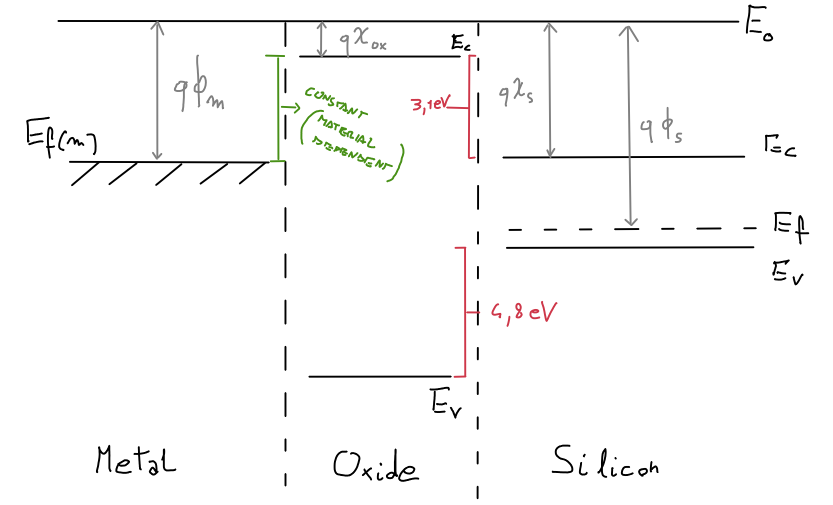
\includegraphics[width=0.7\textwidth]{mos_separate_material.png}\\
\raggedright

We start considering the 3 material isolated from each other under th.eq.\\
We will refer $E_{f(m)}\simeq E_{c}^{Si}$. we have olso to introduce the vacuum level and so electron affinity for oxide and silicon, metal work function, and silicon work function. From this data we can say that the metal we need is Al in order to mantain $E_{f(m)}\simeq E_{c}^{Si}$.\\
We olso underlined in red the potential barrier created by the oxide for holes and electrons.\\

\begin{wrapfigure}{i}{0pt}
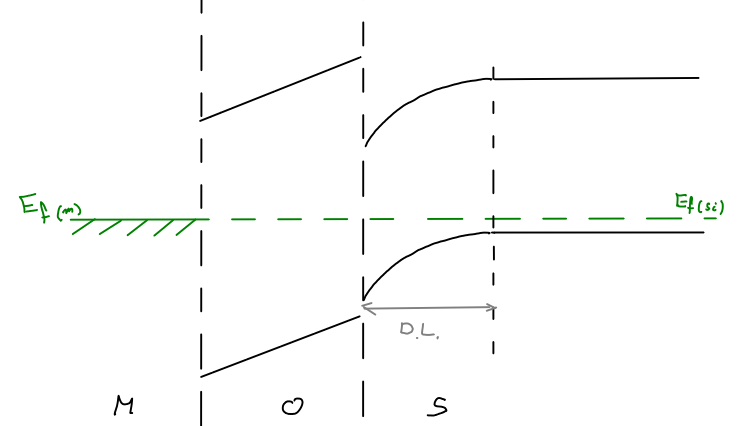
\includegraphics[width=0.5\textwidth]{mos_theq.png}
\end{wrapfigure}

We put the 3 materials in contact after a while we will have a single Fermi-level all over the device and we can say that far from the contact p-Si will be at equilibrium.\\
$E_{f(m)}$ will move downwards toghether with $E_c^{ox}$ since the distance $E_{f(m)}-E_c^{ox}$ is constant (material dependent) as $E_{gap}^{ox}$ .
We have discontinuity of F, for Gauss law $\varepsilon_{ox}F_{ox}=\varepsilon_{Si}F_{Si}\rightarrow F_{ox}=3F_{Si}(0)$. We have a linear band banding in the oxide for the hp of idealty of the dialectric and a parabolic band banding (that means a linear F) in the Si.\\
We have 2 voltage drops over the silicon and over the metal that define $V_s+V_{ox}=\phi_{bi}$.
If we apply a $V>0$ at the gate we push $E_{f(m)}$ downwards creating a higher band banding both in oxide and silicon, this band banding will increase both $V_{ox}$ and $V_{s}$ so assuming that the bulk keeps th.eq we can write the following equation
\begin{equation}
V_{G}+\phi_{bi}=V_s+V_{ox}
\end{equation}
%------------------------------------------------------------------------%
\subsection{Flat band regime}
%------------------------------------------------------------------------%
\begin{wrapfigure}{i}{0pt}
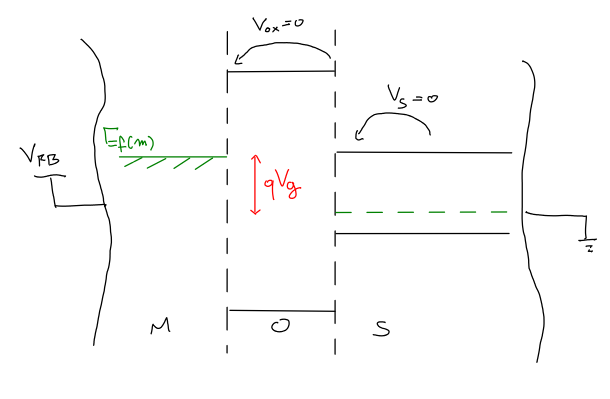
\includegraphics[width=0.5\textwidth]{mos_vfb.png}
\end{wrapfigure}

If we apply $V_G=-\phi_{bi}$ from the previous equation we have that $V_s=V_{ox}=0$ and a separation $E_{f(m)}-E_{f(Si)}=qV_G$.\\
This is the so called Flat-band condition of the mos capacitor 
\begin{equation}
V_{FB}=-\phi_{bi}
\end{equation}
Is defined as the voltage to apply at the gate to have all bands flat.\\
now we can re-write the balance of voltages as
\begin{equation}
V_G-V_{FB}=V_s+V_{ox}
\end{equation}
%------------------------------------------------------------------------%
\subsection{Accumulation regime}
%------------------------------------------------------------------------%
\centering
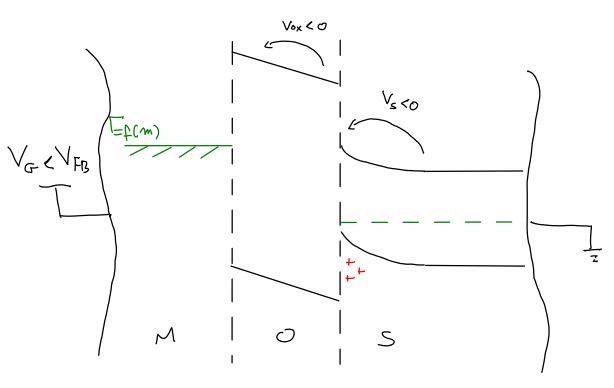
\includegraphics[width=0.5\textwidth]{mos_accum.png}\\
\raggedright


If $V_G<V_{FB}$ bands band upwards we have more holes concentration at the interface between Si-Ox than the doping concentration. \\
This is calle the accumulation regime.
%------------------------------------------------------------------------%
\subsection{Deplition regime} 
%------------------------------------------------------------------------%
\centering
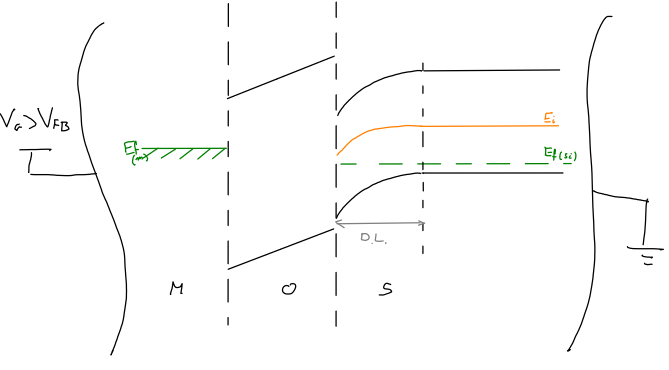
\includegraphics[width=0.5\textwidth]{mos_depl.png}\\
\raggedright

With $V_G>V_{FB}$ we have in silicon a depletion region so we are in the depletion regime of the mos capacitor.
%------------------------------------------------------------------------%
\subsection{Weak inversion condition}
%------------------------------------------------------------------------%
\centering
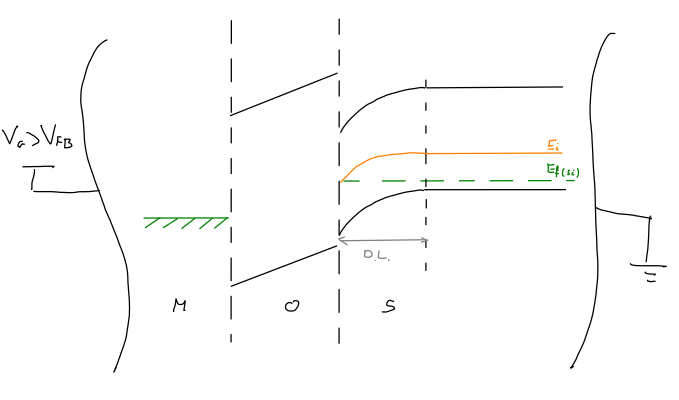
\includegraphics[width=0.5\textwidth]{mos_weak.png}\\
\raggedright

If we further increase $V_G>>V_{FB}$ we arrive at the condition that the intrinsic Fermi level at the surface reaches the Fermi level ($E_f=E_i$).\\
From now on if we slightly increase the voltage we will have more electrons than holes at the interface. This is the condition for weak inversion condition.\\
%------------------------------------------------------------------------%
\subsection{Strong inversion regime}
%------------------------------------------------------------------------%
If we continue to increase the voltage applied we will reach the strong inverson regime that is characterized by $(E_i-E_f)|_{interface}=-(E_i-E_f)|_{bulk}$ so the concentration of electrons at the interface is equal to the doping concentration in the bulk.

%------------------------------------------------------------------------%
\section{Electrostatics}
%------------------------------------------------------------------------%
\centering
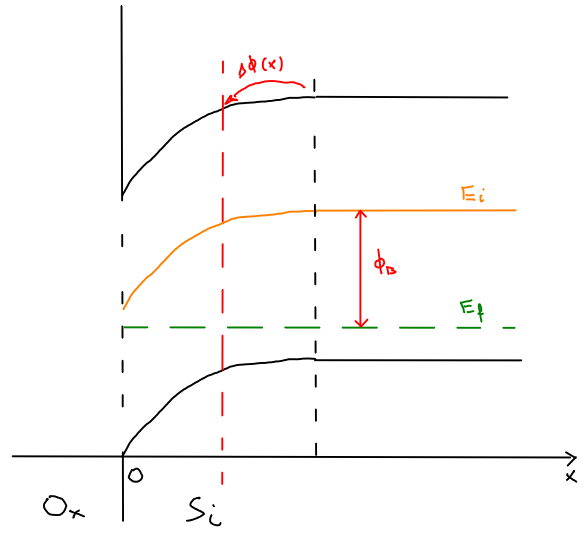
\includegraphics[width=0.5\textwidth]{mos_electrostatic.png}\\
\raggedright

We have to solve the Poisson equation $\frac{d^2\phi}{dx^2}=-\frac{q}{\varepsilon_{Si}}(p-n-N_a^-)$ only in the substrate.\\
We define $\phi_B=E_f-E_i=[E_f=0]=-\frac{kT}{q}\ln(N_a/N_i)$ the electrostatic potential of the bulk far away from the interface and we take $E_f$ that is costant as the reference energy level 0.\\
We introduce olso $\Delta \phi (x)=\phi(x)-\phi_B$  that is the change of the electrostatic potential wrt the bulk;$\Delta \phi (W_d)=0$ and $\Delta \phi (0)=V_s$.\\
\vspace{5mm}
Now we have to write $p-n-N_a^-$ as function of $\phi(x)$.\\
For electrons we can say that $n=n_ie^{(E_f-E_i)/kT}$ if we multiply and divide by q we get $n=n_ie^{q\phi(x)/kT}$ same for holes as $p=n_ie^{-q\phi(x)/kT}$. Electrons and holes in the bulk are $n_0=n_ie^{q\phi_b/kT}$ and $p_0=n_ie^{-q\phi_b/kT}$. From this 4 equation we can write that 
\begin{equation}
n=n_0e^{q\Delta \phi/kT} \ \ \ \ \ \ \ \ p=p_0e^{-q\Delta \phi/kt}
\end{equation}
In the bulk we can say ythat $p_0=n_0+N_a$ so 
\begin{equation}
N_a=p_0-n_0
\end{equation}
Now Poisson equation becomes 
\begin{equation}
\frac{d^2\phi}{dx^2}=-\frac{q}{\varepsilon_{Si}}(p_0e^{-q\Delta \phi/kt}-n_0e^{q\Delta \phi/kT}-p_0+\frac{n_i^2}{p_0})
\end{equation}
Until now the only approximation we have made is the M-B. Now we consider the complete ionization approximation $p_0\simeq N_a$. And we make a change of variable 
\begin{equation}
\frac{d^2\phi}{dx^2}=-\frac{q}{\varepsilon_{Si}}(N_ae^{-q\Delta \phi/kt}-\frac{n_i^2}{N_a}e^{q\Delta \phi/kT}-N_a+\frac{n_i^2}{N_a})
\end{equation}
\begin{equation}
d(\frac{d\phi}{dx})=-\frac{q}{\varepsilon_{Si}}(N_ae^{-q\Delta \phi/kt}-\frac{n_i^2}{N_a}e^{q\Delta \phi/kT}-N_a+\frac{n_i^2}{N_a})dx
\end{equation}
\begin{equation}
\frac{d\phi}{dx}d(\frac{d\phi}{dx})=-\frac{q}{\varepsilon_{Si}}(N_ae^{-q\Delta \phi/kt}-\frac{n_i^2}{N_a}e^{q\Delta \phi/kT}-N_a+\frac{n_i^2}{N_a})dx\frac{d\phi}{dx}
\end{equation}
Now we integrate one time this expression. The first member is like f(x)f'(x) so the result is $-1/2(\frac{d\phi}{dx})^2$. Integrating olso the second member and gathering the common terms the equation we get
\begin{equation}
(\frac{d\Delta \phi }{dx})^2=\frac{2kTN_a}{\varepsilon_{si}}\left(e^{-q\Delta \phi/kT}+\frac{q\Delta \phi}{kT}-1+\frac{n_i^2}{N_a^2}(e^{q\Delta \phi/kT}-\frac{q\Delta \phi}{kT}-1)\right)=F^2(x)
\end{equation}
For Gauss law $F_s=F(0)=-\frac{Q_s}{\varepsilon_{si}}$ (and olso that $\Delta \phi (0)=V_s$ )from this relation and the previous equation we get
\begin{equation}
Q_s=\pm\sqrt{2kTN_a\varepsilon_{si}}\left(e^{-qV_s/kT}+\frac{qV_s}{kT}-1+\frac{n_i^2}{N_a^2}(e^{qV_s/kT}-\frac{qV_s}{kT}-1)\right)^{1/2}
\end{equation}
We already know the total charge in the substrate for all working regimes.\\
%------------------------------------------------------------------------%
\subsection{Dominant terms in the solution of Poisson equation}
%------------------------------------------------------------------------%
\centering
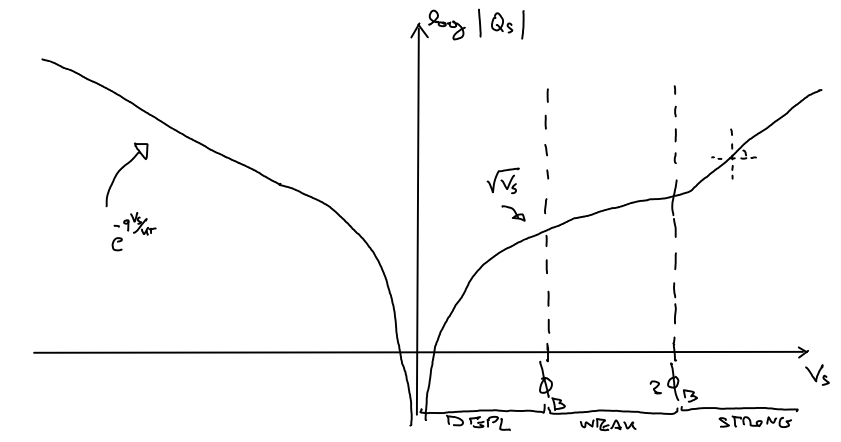
\includegraphics[width=0.5\textwidth]{logqVs.png}\\
\raggedright

To better undestand this formula let's analyse all working regime separately and draw a $\log |Q_s| - V_s$ graph.\\

\vspace{5mm}
In accumulation regime when $V_s<0$ we have that $Q_s\simeq \sqrt{2kTN_a\varepsilon_{si}}e^{-\frac{qV_s}{2kT}}$. So in the graph we see a straight line dependence. We can say that the term
\begin{equation}
e^{\frac{-qV_s}{kT}}\rightarrow h_{sub}
\end{equation} 
in the solution of the Poisson equation is the term that takes into account for hole concentration in the substrate.\\

\vspace{5mm}
In the depletion regime $0<V_s<2|\phi_b|$ we have to consider two dominant term: $\frac{qV_s}{kT}$ and $\frac{n_i^2}{N_a^2}e^{\frac{qV_s}{kT}}$. If we evaluate the second term at $2|\phi_b|$ we get 1 so it's negligible and therefore the first term is predominant. In this regime
\begin{equation}
Q_s\simeq -qN_a\sqrt{\frac{2\varepsilon_{Si}}{q}\frac{1}{N_a}V_s}
\end{equation}
that is the charge of the depletion layer.\\

\vspace{5mm}
In strong inversion $Q_s\simeq \sqrt{2kTN_a\varepsilon_{si}}\frac{n_i^2}{N_a^2}e^{\frac{qV_s}{2kT}}$ so we can say that the term
\begin{equation}
\frac{n_i^2}{N_a^2}e^{\frac{qV_s}{kT}}\rightarrow e_{sub}
\end{equation}
in the solution of the Poisson equation is the term that takes into account electrons in the substrate.\\

%------------------------------------------------------------------------%
\subsection{Total charge in function of gate bias}
%------------------------------------------------------------------------%
We want $Q(V_g)$ ; to have that expression we need to remember that $V_g-V_{fb}=V_s+V_{ox}$ but we can write $V_{ox}=F_{ox}t_{ox}=\frac{\varepsilon_{Si}F_{Si}}{\varepsilon_{ox}}t_{ox}=-Q(V_s)/C_{ox}$ so $V_g-V_{fb}=V_s-\frac{Q_s}{C_{ox}}$ using this expression and $Q_s=Q_s(V_s)$ we can get what we want.\\
We will plot olso the 2 graphs $V_s-V_g$ and $|Q_s|-V_g$.\\

\centering
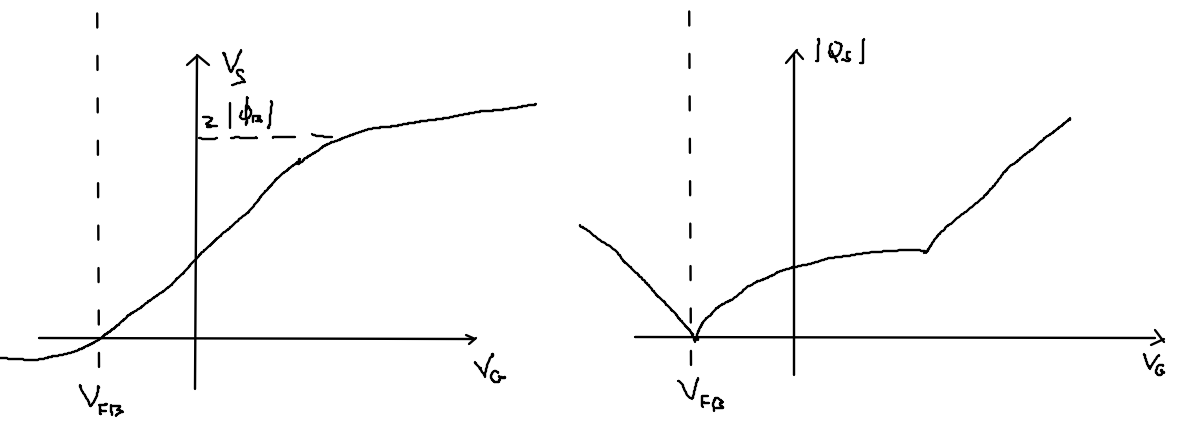
\includegraphics[width=0.5\textwidth]{qvs.png}\\
\raggedright


We will take as reference point the flat band condition where $Q_s=0$ and $V_s=0$.\\

\vspace{5mm}
For $V_s<0$ we said that  $Q_s\simeq \sqrt{2kTN_a\varepsilon_{si}}e^{-\frac{qV_s}{2kT}}$ so we get that
\begin{equation}
V_g-V_{fb}=V_s-\frac{\sqrt{2kTN_a\varepsilon_{si}}}{C_{ox}}e^{-\frac{qV_s}{2kT}}
\end{equation} 
we can neglect $V_s$ beacuse it's negligible wrt the exponential term so we get 
\begin{equation}
V_s\simeq-\frac{2kT}{q}\ln\left(\frac{C_{ox}(V_{fb}-V_g)}{\sqrt{2kTN_a\varepsilon_{si}}} \right) \ \ \ \ \ \ Q_s\simeq C_{ox}(V_{fb}-V_g)
\end{equation}
a small variation of $V_g$ let $V_s$ move not so much due to the exponential increase of the charge in the bulk and a consequent big field in the oxide; we are not far from a metal plate capacitor.\\

\vspace{5mm}
For $0<V_s<\phi_b$ we get that $Q_s\simeq \sqrt{2qN_a\varepsilon_{Si}V_s}$ so we get the following equation (that we don't solve)
\begin{equation}
V_g-V_{fb}=V_s+\frac{\sqrt{2qN_a\varepsilon_{Si}V_s}}{C_{ox}}
\end{equation}

\vspace{5mm}
For weak inversion $\phi_b<V_s<2\phi_b$ we can consider both dominants terms 
getting the following equation 
\begin{equation}
V_g-V_{fb}=V_s+\frac{\sqrt{2\varepsilon_{si}kTN_a}}{C_{ox}}\left(\frac{qV_s}{kT}+\frac{n_i^2}{N_a^2}e^{qV_s/kT} \right)^{1/2}\simeq V_s+\frac{\sqrt{2\varepsilon_{si}kTN_a}}{C_{ox}}\sqrt{\frac{qV_s}{kT}}\left(1+\frac{n_i^2}{2N_a^2}e^{qV_s/kT}\frac{kT}{qV_s}\right)
\end{equation}
using Taylor expansion we get an exponential dependance on $V_g$ of the e charge (that is the second term). Form this dependace we will get the sub-th current of the mos capacitor.\\

\vspace{5mm}
For strong inversion we get 
\begin{equation}
V_g-V_{fb}=V_s+\frac{\sqrt{2\varepsilon_{si}kTN_a}}{C_{ox}}\frac{n_i}{N_a}e^{qV_s/2kT}
\end{equation}
remembering that $\frac{n_i^2}{N_a^2}e^{q2|\phi_b|/kT}=1$ we can say that $\frac{n_i}{N_a}=e^{-q2|\phi_b|/2kT}$ so we can write that 
\begin{equation}
V_g-V_{fb}=V_s+\frac{\sqrt{2\varepsilon_{si}kTN_a}}{C_{ox}}e^{\frac{q(V_s-2|\phi_b|)}{2kT}}
\end{equation}
So we get $V_s$ and making a rought approx of $V_s\simeq 2|\phi_b|$ olso $Q_s$
\begin{equation}
V_s=2|\phi_b|+\frac{2kT}{q}\ln \left(\frac{C_{ox}(V_g-V_{fb}-V_s)}{\sqrt{2\varepsilon_{si}kTN_a}} \right) \ \ \ \ \ \ Q_s=-C_{ox}(V_g-V_{fb}-2|\phi_b|)
\end{equation}
The approximation means that entering in storng inversion we get a maximum depletion layer and a maximum depletion charge
\begin{equation}
W_d^{max}=\sqrt{\frac{2\varepsilon_{si}}{qN_a}2|\phi_b|} \ \ \ \ \ \ \ \ \ Q_{dep}^{max}=-\sqrt{2\varepsilon_{si}qN_a2|\phi_b|}
\end{equation}
we increase the charge of electrons not that of the depletion layer.\\
The $V_g$ at witch we enter in the strong inversion is $V_g-V_{fb}=2|\phi_b|+\frac{|Q_{dep}^{max}|}{C_{ox}}$ that is called threshold voltage of the mos capacitor that is 
\begin{equation}
V_t=V_{fb}+2|\phi_b|+\frac{|Q_{dep}^{max}|}{C_{ox}} \ \ \ \rightarrow Q_{inv}=Q_s-Q_{dep}^{max}=-C_{ox}(V_g-V_t)
\end{equation}

%------------------------------------------------------------------------%
\section{Small signal capacitance}
%------------------------------------------------------------------------%
We want to study the small signal capacitance of the MOS capacitor that is a non linear device so we want $C_g=-\frac{dQ_s}{dV_g}$ the change of charge over the change of voltage.\\
We can guess the behaviour of $C_g$ using the expression $V_g-V_{fb}=V_s-Q_s/C_ox$ and calculating the derivative wrt $d(-Q_s)$ we get
\begin{equation}
\frac{dV_g}{d(-Q_s)}=\frac{dV_s}{d(-Q_s)}+\frac{1}{C_ox}
\end{equation}
that is 
\begin{equation}
\frac{1}{C_g}=\frac{1}{C_s}+\frac{1}{C_{ox}}
\end{equation}
The total gate capacitance can be expressed by the series of 2 capacitive terms one fixed ($C_{ox}$) one variable (that is the substrate capacitance $C_s$). From this we know that $C_g$ has an upper limit of $C_{ox}$.\\
Let's analise the small signal capacitance in the various regime.\\

\subsection{in accumulation regime}
We derivate the charge of the accumulation region obtaining 
\begin{equation}
C_s=\sqrt{2kTN_a\varepsilon_{si}}e^{-\frac{qV_s}{2kT}}\frac{q}{2kT}=Q_s/\frac{2kT}{q}
\end{equation}
Knowing $Q_s(V_g)$ we get 
\begin{equation}
C_s=\frac{C_{ox}(V_{fb}-V_g)}{2kT/q}
\end{equation}
This is $>>C_{ox}$ if $V_{fb}-V_g>>2kT/q$. So from flat band to minus infinite the capacitance increases and becomes similar to $C_{ox}$. We are close to a metal plate capacitor.\\

\subsection{in flat band condition}
We have to include in the Q expression both electrons and holes so $Q_s=\sqrt{2kTN_a\varepsilon_{si}}(e^{\frac{-qV_s}{kT}}+\frac{qV_s}{kT}-1)^{1/2}$.\\ If we make the Taylor expansion of the exponential term around 0 we get $Q_s=-V_s\sqrt{\frac{\varepsilon_{si}q^2N_a}{kT}}$ so 
\begin{equation}
C_s=\frac{d(-Q_s)}{dV_s}=\frac{\varepsilon_{si}}{\sqrt{\frac{\varepsilon_{si}kT}{q^2 N_a}}}=\frac{\varepsilon_{si}}{L_D}
\end{equation}
we can recognise the Dybae lenght in the expresison we can interpretate this result as this ; the holes (majority) screen a perturbation of the electric field form the gate like a step increase of doping concentration.\\
This capacitance and the oxide capacitance are comparable.\\

\subsection{in depletion regime}
In depletion regime we have a charge $Q_s=-\sqrt{2\varepsilon_{Si} q N_a V_s}$ that is the usual expression for the charge in a depletion layer. From the well known realtion $C=\varepsilon_{si}/t_{ox}$ we get 
\begin{equation}
C_g=C_{ox}/\sqrt{1+2C_{ox}^2 \frac{V_g-V_{fb}}{\varepsilon_{si}qN_a}}
\end{equation}
This capacitance decrease quickly near the flat band condition beacuse the contribution related to holes disappears over a few kT/q.\\

\subsection{in strong inversion} 
We have the charge $Q_s=\sqrt{2\varepsilon_{Si}kTN_a}\frac{n_i}{N_a}e^{\frac{qV_s}{2kT}}$ so making the derivate we reach 
\begin{equation}
C_s=\frac{|Q_s|}{2kT/q}=C_{ox}\frac{(V_g-V_{fb}-2|\phi_b|)}{2kT/q}
\end{equation}
Increasing $V_g$ we get a larger capacitance we reach a condition similar to a metal plate capacitance.\\

\centering
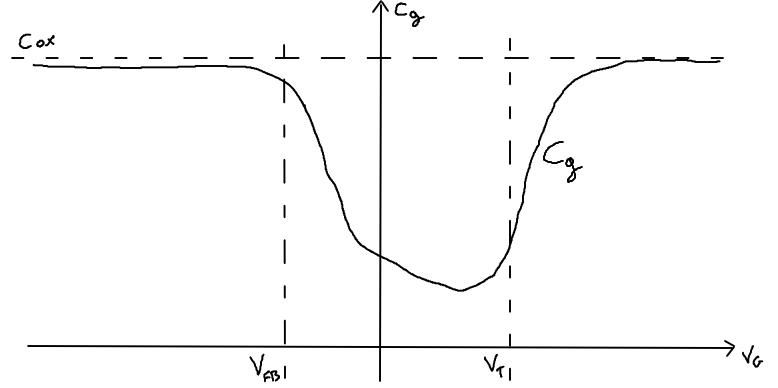
\includegraphics[width=0.35\textwidth]{c-g1.png}\\
\raggedright



%------------------------------------------------------------------------%
\section{Frequency regimes}
%------------------------------------------------------------------------%
\centering
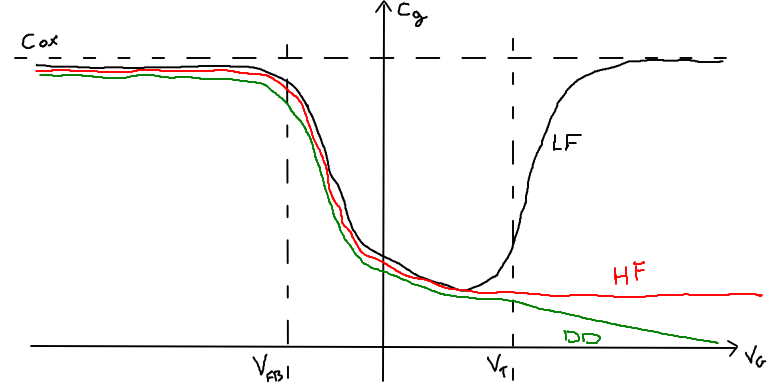
\includegraphics[width=0.7\textwidth]{c-gtot.png}\\
\raggedright

Let's look more colsely to the substrate during the different regimes when we apply a small signal to the gate.\\

\vspace{5mm}
{\bf In accumulation regime}\\
$\overline{V_g}<V_{fb}$ if we move the gate of $\delta V_g>0$ we are removing h from the silicon surface to the substrate. Vice-versa with $\delta V_g<0$ we move h from the substrate to the silicon surface.\\
This is a modulation of majority carriers concentration so it happens in a very short time in the order of the dialectric relaxation time.\\

\vspace{5mm}
{\bf In weak inversion}\\
$V_{fb}<\overline{V}<V_t$ we have a depletion region with a certain voltage drop $V_s$ and an exposed negative charge at the surface.\\
With a $\delta V_g>0$ we slightly increase the width of the depletion layer so we are removing holes from the edge of the depletion layer to the substrate. With $\delta V_g<0$ we reduce the depletion layer so we add h from the substrate to the depletion layer to neutralize the exposed charge.\\
Olso here we modulate the majority carrier so this is a process that have as time constant the dialectric relaxation time.\\

\vspace{5mm}
{\bf Strong inversion}\\
Depletion layer at the maximum expansion at the silicon surface we have a lot of electrons.\\ 
Appling $\delta V_g$ we modulate e concetration this electrons cannot came from the contact that exchange only majority they have to be created by generation processes.\\

%------------------------------------------------------------------------%
\subsection{Low frequency regime}

\begin{wrapfigure}{i}{0pt}
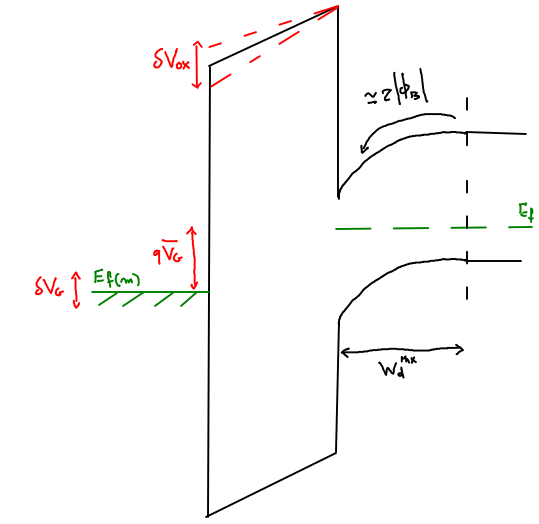
\includegraphics[width=0.4\textwidth]{lfbd.png}
\end{wrapfigure}
The time constant for the generation process in strong inversion can be extracted from the generation current $J_g=q\frac{n_i}{2\tau_0}W_d^{max}$ that is the total current that can be created per unit time per unit area. The charge of the depletion layer is $Q_{dep}=qN_aW_d^{max}$ the time for generate this charge is 
\begin{equation}
\tau_g=\frac{Q_{dep}}{J_g}=2\tau_0N_a/n_i
\end{equation}
$\tau_g$ is technology dependent and very big in the order of seconds.\\
Only if the signal has a frequence much lower than $\tau_g$ ($f<1Hz$) we have the ideal charachteristic seen before.\\
Looking at the band diagram a movement of $\delta V_g$ moves $E_{f(m)}$ upwards or downwards. With a $\delta V_g>0$ we have to increase the total voltage drop but the dependance with $V_{sub}$ is very weak so $\delta V_s\simeq 0$ and we modulate only the voltage drop over the oxide (under charge sheet approximation that we will see in next chapter) $\delta V_g\simeq V_{ox}$


%------------------------------------------------------------------------%
\subsection{High frequency regime}

\begin{wrapfigure}{i}{0pt}
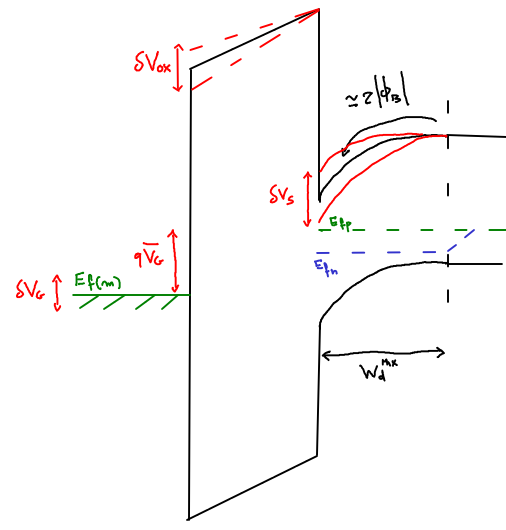
\includegraphics[width=0.4\textwidth]{hfbd.png}
\end{wrapfigure}
For signals with high frequency ($f>1Hz$) we cannot change electron concentration so we can only add or remove holes at the substrate making the depletion layer bigger or smaller.\\ 
The graph of $C_g$ remains constant form the threshold voltage on.\\
The total capacitnace depends on the frequency of the small signal we are appling.\\
Here the modulation of $\delta V_g$ can't modulate the electron concentration at the surface of silicon. There is a modulation of the depletion layer so $\delta V_s$ but for the continuity of the electric field olso $\delta V_{ox}$ have to change in a comparable manner. With the downwards band banding we have to keep constant the distance with $E_{fn}$ with the conduction band so our substrate is no longer at th.eq. This triggers GR processes that tends to move the system back in the th.eq of low freqeuncy.
$E_{fn}$ is constant over the depletion layer and merges with $E_{fp}$ in the quasi neutral region of the device. We have a flow of electrons from the substrate to the surface similar to the pn-j reverse current.\\

%------------------------------------------------------------------------%
\subsection{Deep deplition}

\begin{wrapfigure}{i}{0pt}
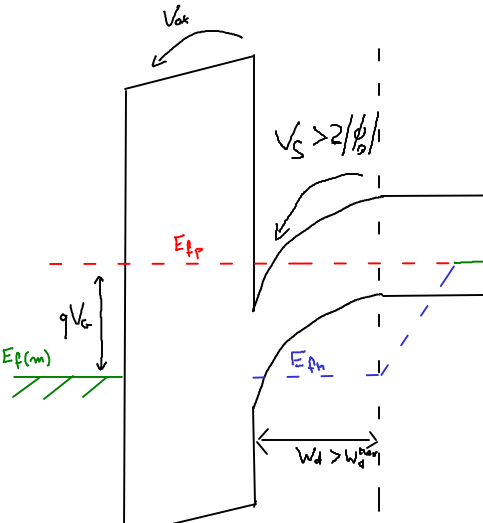
\includegraphics[width=0.4\textwidth]{ddcond.png}
\end{wrapfigure}

If we consider a step increase of the gate voltage form 0 to $\overline{V}_g>V_t$ we don't give the time to the system to create electrons so we get a super wide depletion layer $W_d>>W_d^{max}$. This is called deep depletion condition of the MOS capacitor and it's a large signal regime.\\
If we apply on this step increase a $\delta V_g$ this will modulate the width of the depletion layer (in low and high freqence too) beacuse we don't have electron at the interface. The capacitance is $C_s=C_{dep}=\varepsilon_{si}/W_d$ so the total capacitance will decrease over V.\\
$W_d$ is related to $V_s$ so $W_d>W_d^{max}$ means $V_s>2|\phi_b|$ the conduction band can bend even below the fermi level but we have to keep the condition of no electrons at the interface so we have the split in the two Fermi level for electrons and holes. Small voltage drop ove the oxide due to big voltage drop over the substrate.\\
GR processes will pull the system to the LF regime in order to restore the equilibrimu so with a $Q_{inv}$ of electrons at the surface.\\

\begin{wrapfigure}{i}{0pt}
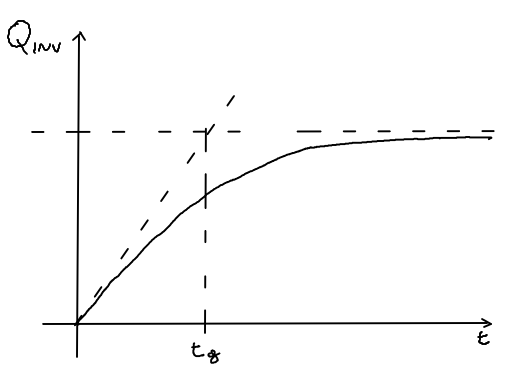
\includegraphics[width=0.3\textwidth]{qinv.png}
\end{wrapfigure}

Let's study the behaviour in time of this charge under the simplifing assumption that $Q_s$ remains constant: so by S-R-H statisic 
\begin{equation}
\frac{dQ_{inv}}{dt}=-qG[W_d(t)-W_d^{max}]=-q \frac{n_i}{2\tau_0}[W_d(t)-W_d^{max}]
\end{equation}
but $Q_s=Q_{inv}+Q_{dep}=Q_{inv}-qN_aW_d(t)$ from here we get that $W_d(t)=(Q_{inv}-Q_s)/(qN_a)$ where $Q_s$ is a constant so we get the following differential equation
\begin{equation}
\frac{dQ_{inv}}{dt}=\frac{n_i}{2\tau_0N_a}Q_{inv}+\frac{qn_i}{2\tau_0}[\frac{Q_s}{qN_a}+W_d^{max}]
\end{equation}
that is a simple first order differential equation which solution is
\begin{equation}
Q_{inv}(t)=[Q_s+qN_aW_d^{max}][1-e^{t/t_g}] \ \ \ \ \ \ t_g=\frac{2\tau_0N_a}{n_i}
\end{equation}
so an exponential increase of the charge with a time constant $t_g$


%------------------------------------------------------------------------%
\section{MOS capacitor with ring}
%------------------------------------------------------------------------%
\centering
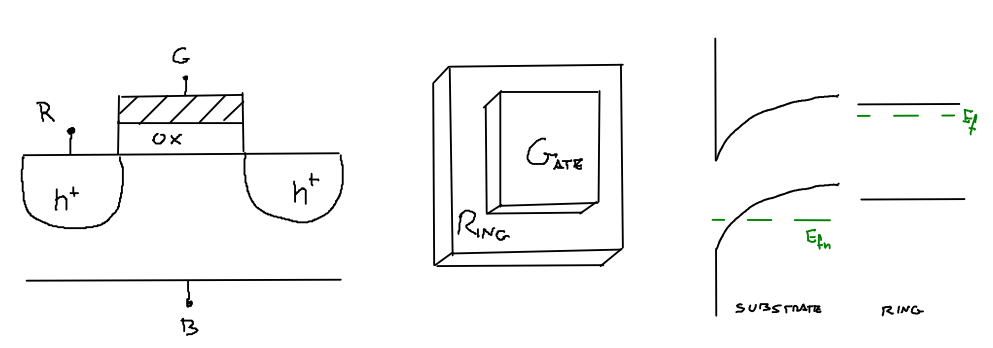
\includegraphics[width=0.7\textwidth]{ring.png}\\
\raggedright
We want to modify the structure adding a contact that can provide a lot of electrons. This contact is calle ring it's $n^+$ doped. With $V_g>V_t$ $E_{fn}$ goes down but the Fermi level in the ring is higher than it so there is a flow of electrons from the ring to the substrate with a time constant similar to the transient time from the 2 zones of the electrons.\\

%------------------------------------------------------------------------%
\subsection{Split C-V curve}
\begin{wrapfigure}{i}{0pt}
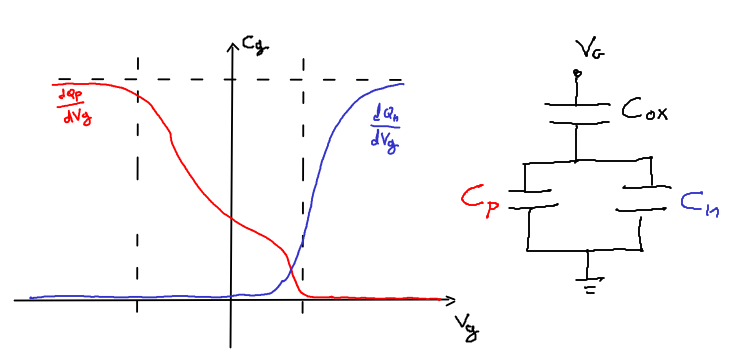
\includegraphics[width=0.5\textwidth]{splitcv.png}
\end{wrapfigure}
With this structure it's possible to measure the current of e and h indipendently and split the 2 contributions.\\
Let's assume that in accumulation regime and weak inversion we modulate only $dQ_p$ no $dQ_n$ flow so the capacitance is only $\frac{dQ_p}{dV_g}=C_g$ beacuse $\frac{dQ_n}{dV_g}=0$.
At stong inversion we modulate only electrons beacuse we reach the maximum width of the depletion layer so $\frac{dQ_p}{dV_g}=0$ and $\frac{dQ_n}{dV_g}=C_g$.\\ In this way we are splitting the total gate capacitance in 2 contributions due to holes and electrons.\\


%------------------------------------------------------------------------%
\subsection{Electrostatic}
%------------------------------------------------------------------------%
\centering
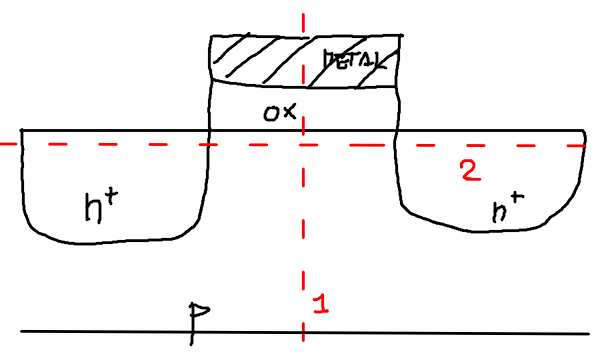
\includegraphics[width=0.35\textwidth]{sections.png}\\
\raggedright

Beacuse the MOS capacitor is an intrinsic 2D device we have to study the electrostatics in the 2 directions of the graph. \\ 
We are not intrested in polrization with $V_r<0$ beause this will make the pn junction in forward bias.\\


%------------------------------------------------------------------------%
\subsubsection{$\rightarrow V_r=V_g=0$}

\centering
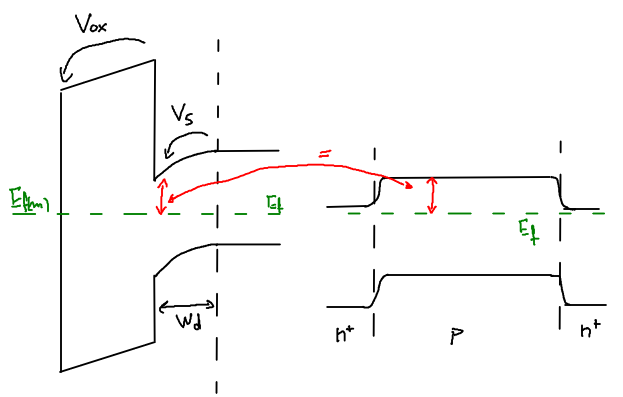
\includegraphics[width=0.7\textwidth]{theqmosr.png}\\
\raggedright

We are under th.eq we are not perturbing the device. In crossection 1 we have weak inversion. In crossection 2 we have 1 single Fermi level for th.eq from crossection 1 we know the distance between the conduction band and $E_f$ in the substrate. The region under the gate in graph 2 is depleted


%------------------------------------------------------------------------%
\subsubsection{$\rightarrow V_r=0 \ \ \  V_g=V_t$}

\centering
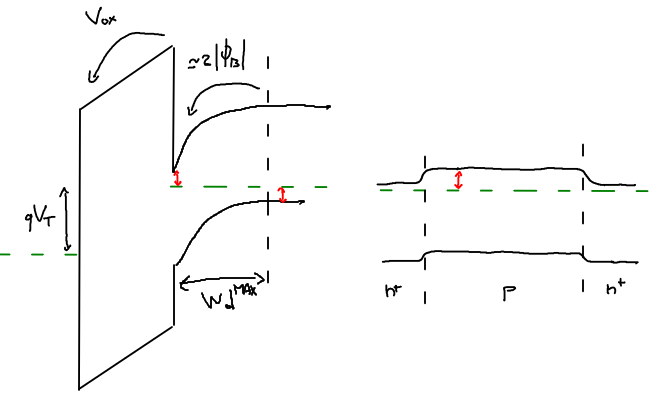
\includegraphics[width=0.7\textwidth]{what1.png}\\
\raggedright

First graph is the one we have already seen. In crossection 2 we make the same consideration as before.


%------------------------------------------------------------------------%
\subsubsection{$\rightarrow V_r>0 \ \ \ V_g=0$}

\centering
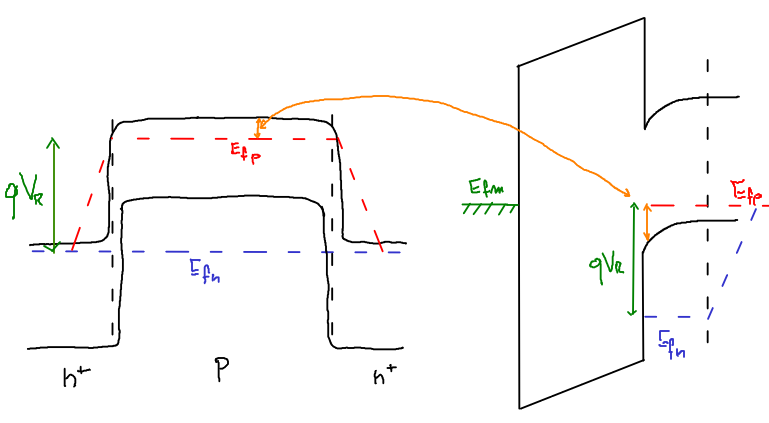
\includegraphics[width=0.7\textwidth]{what2.png}\\
\raggedright

We have no change in crossection 1 wrt the first case.
For second crossection we have to set the distance $E_c-E_f$ under the gate in accord to the first graph. In the $n^+$ region we are applying a potential that bands the band downwards by an amount $qV_r$ giving a large band banding and so a separation of the Fermi levels.\\
The quasi Fermi level for electrons has to stay constant for simmetry $E_{fp}$ changes.\\
Form this we have to modify graph 1 where $E_{fn}$ is moved downwards by an amount $qV_r$ (doing this we do not change the electrostatic beacuse the electron concetration was already negligible so no other modifications in the band banding are needed).\\

%------------------------------------------------------------------------%
\subsubsection{$\rightarrow V_r>0 \ \ \  V_g=V_t$}
Crossection 1 same as the case of $V_r=0 \ \ V_g=V_t$ with the same step of before we get the separation of the quasi Fermi levels in the first graph and the same graph for crossection 2 of the previous case.\\
In this case we are no more in strong inversion due to the shift downwards of $E_{fn}$ of $qV_r$. To gain the strong inversion regime we have to apply a stornger gate bias $V_g=V_t'$ to have $V_s=2|\phi_b|+V_r$ and of course a wider depletion layer.\\

\centering
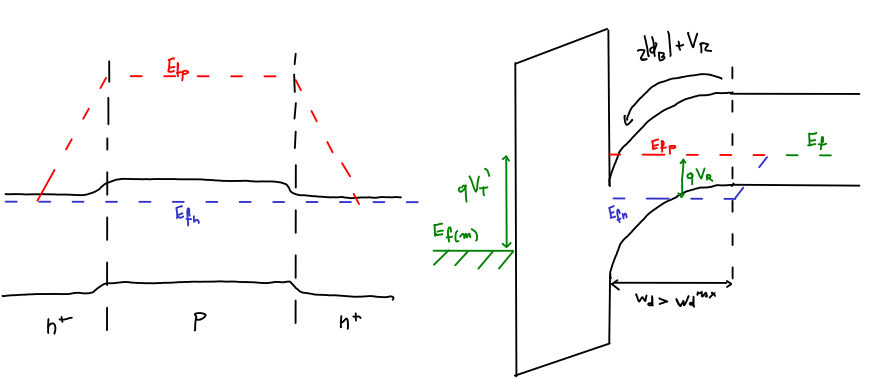
\includegraphics[width=0.77\textwidth]{what3.png}\\
\raggedright
We prolong the depletion regime applying $V_r>0$ changing the on-set of the strong inversion regime to 
\begin{equation}
V_t'=V_{fb}+2|\phi_b|+V_r+\frac{\sqrt{2\varepsilon_{si}qN_a(2|\phi_b|+V_r)}}{C_{ox}}
\end{equation}
adding and removing $\frac{\sqrt{2\varepsilon_{si}qN_a2|\phi_b|}}{C_{ox}}$ we obtain
\begin{equation}
V_t'=V_t(V_r=0)+V_r+\frac{\sqrt{2\varepsilon_{si}qN_a}}{C_{ox}}[\sqrt{2|\phi_b|+V_r}-\sqrt{2|\phi_b|}]
\end{equation}

\centering
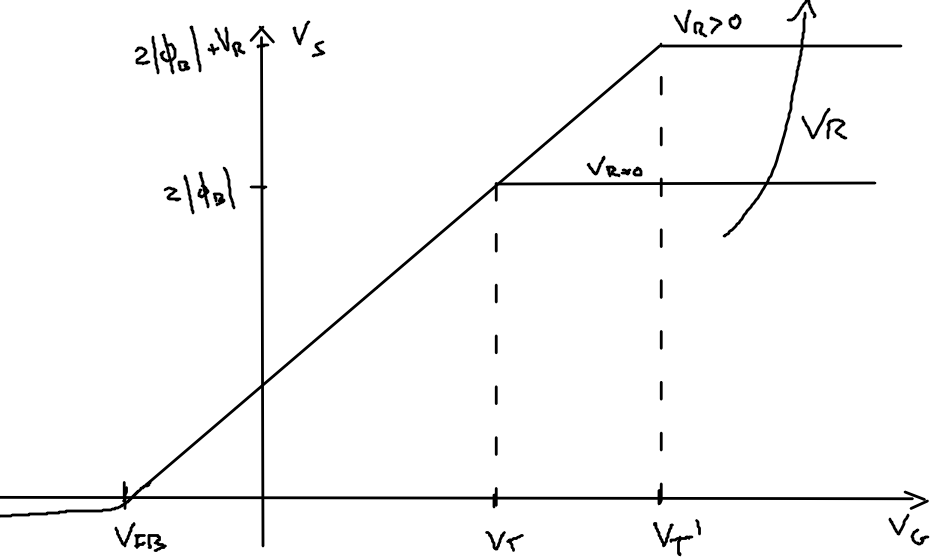
\includegraphics[width=0.4\textwidth]{vtprimo.png}\\
\raggedright

The charge in the substrate will be from the relation $V_g-V_{fb}=V_s-Q_s/C_{ox}$ 
\begin{equation}
Q_{inv}=Q_s-Q_{dep}^{max}=-C_{ox}(V_g-V_{fb}-2|\phi_b|-V_r-|Q_{dep}^{max}|/C_{ox})=-C_{ox}(V_g-V_t')
\end{equation}
In accumulation and strong inversion the MB approximation isn't valid and gives us a big error wrt the FD. Below there are the graph change for the 2 distribution for $C_s-V_g$ and $C_s-V_g$.\\

\centering
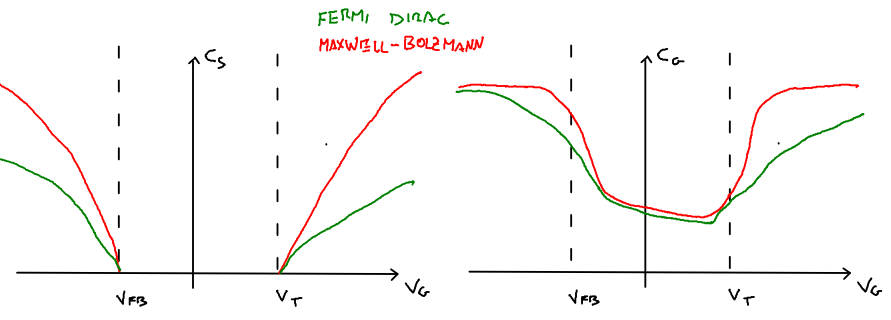
\includegraphics[width=0.6\textwidth]{mbvsfdmos.png}\\
\raggedright


%------------------------------------------------------------------------%
\section{Effects of non idealities}
%------------------------------------------------------------------------%

%------------------------------------------------------------------------%
\subsection{Charge in the oxide}

Charge in the oxide is caused due to spurious states inside the dialectric or difects that trap charges furthermore ageing increase the density of this imperfections.\\
Let's assume a MOS capacitor at the flat band condition with a negative charge sheet at distance x from the gate.\\ 

\centering
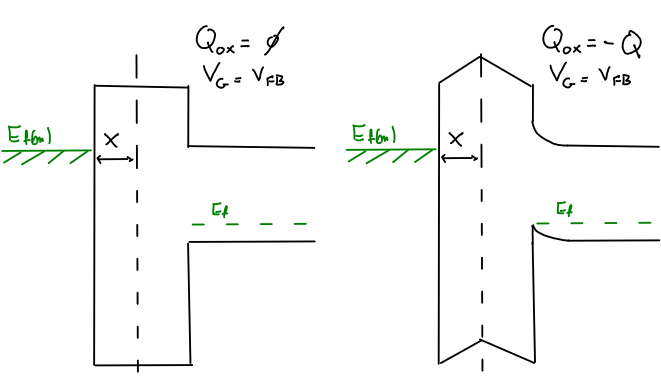
\includegraphics[width=0.6\textwidth]{qinox.png}\\
\raggedright

The negative charge decreases the potential so bands upwards the bands. We have a linear banding beacuse the charge is concentrated in one point.\\
We have a layer of hole at the the substrate and olso a positive charge on the gate (electrostatic induction tends to nihil the charge). The important fact is that $V_s\neq0$ with the flat-band voltage.\\
To recover the flat band state we have to decrease $E_{f(m)}$ so increase the gate voltage; the new flat band voltage will be $V_{fb}'=V_{fb}+\Delta V_g$. With Gauss law we get
\begin{equation}
\Delta V_g=-\frac{Q_{ox}}{\varepsilon_{ox}}x
\end{equation}
This expression can be re-writed introducing the parameter $C_{xg}=\varepsilon_{ox}/x$ the capacitance between x and the gate as
\begin{equation}
\Delta V_g=-\frac{Q_{ox}}{C_{xg}}
\end{equation}
The maximum value for this voltage variation is when $x=t_{ox}\rightarrow C_{xg}=C_{ox}$. This is reasonable result lower the distance higher the electrostatic induction.\\
The above results are general and valid for all working regimes of the MOS capacitor.\\
The effect of this phenomena results in the C-V curve as a shift rightwards if the charge is negative, leftwards if the charge is positive, of $\Delta V_g$.\\
If we get a distribution of charge per unti volume of $\rho$ we get 
\begin{equation}
\Delta V_g=\int_0^{t_{ox}}\frac{x\rho}{\varepsilon_{ox}}dx
\end{equation}

%------------------------------------------------------------------------%
\subsection{Interface states}

\centering
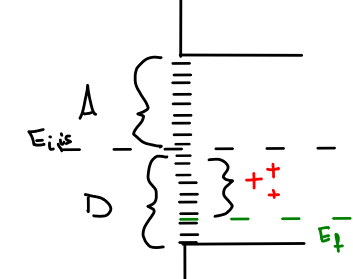
\includegraphics[width=0.2\textwidth]{istafb.png}\\
\raggedright

First we will consider the flat-band condition.\\
Acceptor states are all empty so no charge as the donor states below $E_f$ that are all filled. There are some donor empty that gives us a positive charge (that make the potential higher and so decrease the bands). Following the results of the charge sheet in the oxide we can restore the ideal case by appling a $\Delta V_g= -Q_i/C_{ox}$.\\

\centering
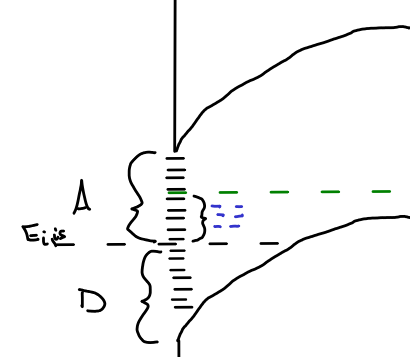
\includegraphics[width=0.2\textwidth]{istasi.png}\\
\raggedright

In strong inversion we have a negative charge exposed that can be compensated with an extra voltage as before but with opposite sign.\\
In accumulation and flat-band regime we have a negative increase so a shift leftwards of the C-V curve for the stron inversion vice versa so we have a strech of the total C-V characteristic.

\centering
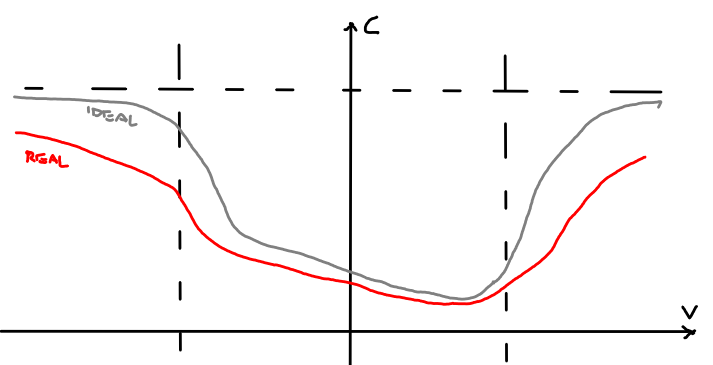
\includegraphics[width=0.5\textwidth]{cvis.png}\\
\raggedright

%------------------------------------------------------------------------%
\section{Impact of polysilicon gate}

The benefit of usign the polisilicon gate comes from a tecnological issues.\\
First way to do ring-MOS was by create a p-substrate, create the $n^+$ regions, let the oxide deposit all over, deposit the gate and then remove by etching the excess of gate and oxide. This type of process is a non self-allign process.\\

\centering
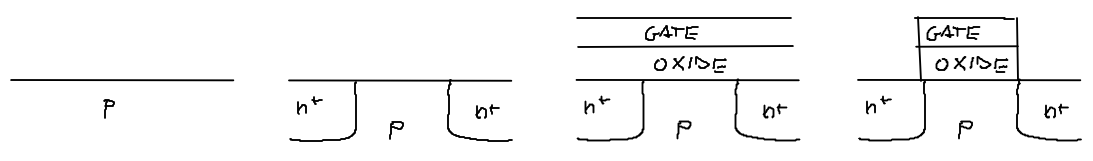
\includegraphics[width=0.65\textwidth]{process1.png}\\
\raggedright

Processes tollerances define where the gate is placed. If the gate is over the $n^+$ zone there will be a big parassite capacitance but on the other hand with the gate far from that zone there will be no control of electrons by the gate.

\centering
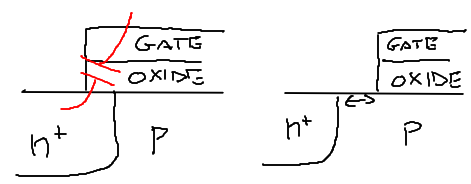
\includegraphics[width=0.25\textwidth]{process1par.png}\\
\raggedright

A better process is : p-substrate, deposit the oxide, deposit the gate, etching excess and than n-dope. This is a self alligned process.\\

\centering
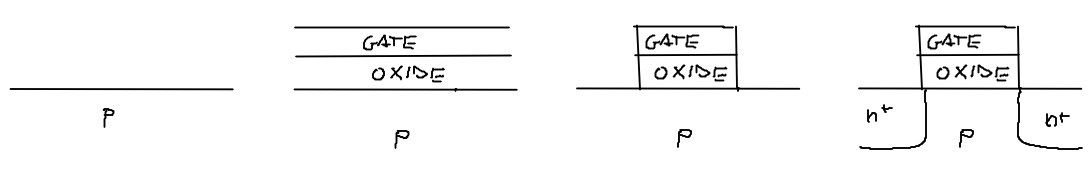
\includegraphics[width=0.65\textwidth]{process2.png}\\
\raggedright

To dope we have to do a heat threatment at 800C so this process does not works with metals (melting point issues) but works with polysilicon.\\
Olso another improvmen comes from the threshold voltage $V_t=V_{fb}+2|\phi_b|+|Q_{dep}^{max}|/C_{ox}$ that with a poly-p-doped gate is $\simeq 0$ but with a n-doped-poly is reduced to $V_t=|Q_{dep}^{max}|/C_{ox}$ beacuse $V_{fb}\simeq -1V$ in this case and $2|\phi_b|\simeq 1V$.\\
The problem with this gate material is that we have to consider the charge as for unit volume not as untit area (we don't have that much electrons as in a metal) so doing we get a depletion layer olso in the gate of $W_d=\sqrt{\frac{2\varepsilon_{si}V_p}{qN_d^g}}$ and so an additional voltage drop $V_p$ and an additional capacitance.\\

\centering
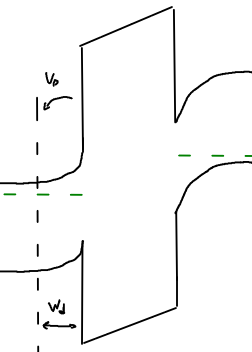
\includegraphics[width=0.25\textwidth]{polygate.png}\\
\raggedright

The voltage ballance is now $V_g-V_{fb}=V_s+V_{ox}+V_p$ deriving wrt $-Q_s$ we get 
\begin{equation}
\frac{1}{C_{g}}=\frac{1}{C_{s}}+\frac{1}{C_{ox}}+\frac{1}{C_{g}}
\end{equation}
The C-V curve doesn't change until strong inversion when this phenomena becomes dominant. We can write that 
\begin{equation}
\frac{1}{C_g}=\frac{2kT/q}{Q_p}+\frac{1}{C_{ox}}+\frac{Q_p}{qN_d^{g}\varepsilon_{si}}
\end{equation}
the last term becomes dominant in strong inversion.\\
This is why we now use again metal for gate (with particular mix with high melting point).\\
































